\documentclass[]{article}

\usepackage[sort&compress,numbers]{natbib}
\bibliographystyle{apsrev4-1}
\usepackage{doi}%<----------
\usepackage{hyperref}

\usepackage{paracol,lipsum}
\usepackage{verse}
\usepackage[margin=.2in]{geometry}
\usepackage{tasks}
\usepackage{exsheets}
\SetupExSheets[question]{type=exam}

\usepackage{amssymb,latexsym}
\usepackage{amsmath,amsbsy,bbm}
\usepackage{epsfig,bm,color}
\usepackage{cjhebrew}
\usepackage{nicefrac}
\usepackage{graphicx,comment}
\usepackage{slashed}
\usepackage{yfonts}
\usepackage{nomencl}
\usepackage{physics}
\usepackage{tikz}
\usepackage[tikz]{bclogo}
\usetikzlibrary{calc,arrows.meta}

%\usepackage{hyperref}
\unitlength=1mm

\usepackage{dutchcal}

\usepackage{calligra}

\DeclareMathAlphabet{\mathcalligra}{T1}{calligra}{m}{n}
\DeclareFontShape{T1}{calligra}{m}{n}{<->s*[2.2]callig15}{}
\newcommand{\scriptr}{\mathcalligra{r}\,}
\newcommand{\boldscriptr}{\pmb{\mathcalligra{r}}\,}

\def\eqref#1{{(\ref{#1})}}

\newcommand{\caf}{\text{\cjRL{b}}}
\newcommand{\helium}{${}^4$He}
\newcommand{\helion}{${}^3$He}
\newcommand{\triton}{${}^3$H}
\newcommand{\ecm}{E_\textrm{\small c.m.}}
\newcommand{\dq}{\mbox{d\hspace{-.55em}$^-$}}
\newcommand{\mpis}{$m_\pi=137~${\small MeV}}
\newcommand{\mpim}{$m_\pi=450~${\small MeV}}
\newcommand{\mpil}{$m_\pi=806~${\small MeV}}
\newcommand{\muh}{\mu_{^3\text{\scriptsize He}}}
\newcommand{\mut}{\mu_{^3\text{\scriptsize H}}}
\newcommand{\mud}{\mu_\text{\scriptsize D}}
\newcommand{\pode}{\beta_{\text{\scriptsize D},\pm1}}
\newcommand{\poh}{\beta_{^3\text{\scriptsize He}}}
\newcommand{\pot}{\beta_{^3\text{\scriptsize H}}}
\newcommand{\com}[1]{{\scriptsize \sffamily \bfseries \color{red}{#1}}}
\newcommand{\eftnopi}{\mbox{EFT($\slashed{\pi}$)}}
\newcommand{\red}[1]{\textcolor{red}{#1}}
\newcommand{\green}[1]{\textcolor{green}{#1}}
\newcommand{\blue}[1]{\textcolor{blue}{#1}}
\newcommand{\drei}[1]{\delta^{(3)}\!\left(#1\right)}
\newcommand{\ddrei}[1]{\delta_{\tiny \Lambda}^{(3)}\!\left(#1\right)}

\newcommand{\ecce}[2]{\paragraph*{Ecce: #1}\texttt{\textcolor{blue}{#2}}}

\newcommand{\tqt}[1]{\begin{flushleft}---\textquotedblleft\textit{#1}\textquotedblright\par\end{flushleft}}
\newcommand{\attrib}[1]{%
\nopagebreak{\raggedleft\footnotesize #1\par}}
\renewcommand{\poemtitlefont}{\normalfont\large\itshape\centering\bf}

\makenomenclature

\begin{document}
\columnratio{0.45}
% ------------------------------------------ LEFT COLUMN ------------------------------------------
\begin{paracol}{2}

\subsection*{\small Aperitif}

\tqt{The structure of dynamical equations is desceptively simple, obfuscating the marvelous phenomena
which they point us to in nature decades and conturies post their conception.}

\begin{tasks}
    \task The goal is the investigation of $N$-body systems and how linked/disentangled they behave with respect to
    their subsystems
    \task The elementary instance we want to analyze--empirically, at fisrt--is the celestial $N$-body
    problem with the trajectories of $M<N$ of its constituents being fixed~(we aim from the start to
    generalize the text-book problem~\cite{Schmid1990,Geiges_2016}~which deals with 3 objects of which 2 are fixed).
    \task Let us tackle the restricted 5-body problem and commence by formulating the pertinent equations of motion.
    We \emph{chose} to fix the orbits of 4 of the 5 objects to circular trajectories about the origin, which is,
    the centre of mass.
    \task The coordinates and the velocity of the 5th object comprise the only degrees of freedom of the system,
    and we choose to start from a Lagrangean formulated in cartesian coordinates as we expect this approach to
    generalize straight-forwardly to larger $N$ and $M$.
\end{tasks}

\switchcolumn

% ------------------------------------------ RIGHT COLUMN ------------------------------------------
\begin{tasks}
    \task
    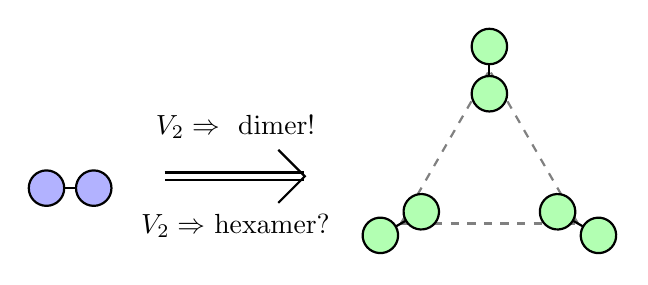
\begin{tikzpicture}[thick,scale=1.5]
\tikzset{math arrow/.style={double distance=2pt, -{Straight Barb[scale=1.1]}}}
% Dimer on the left
\draw (-3,0.3) -- (-2.6,0.3); % connector
\draw[fill=blue!30] (-3,0.3) circle (0.15);
\draw[fill=blue!30] (-2.6,0.3) circle (0.15);

% Arrow to the right
\draw[math arrow] (-2.0,0.4) -- (-0.8,0.4) node[midway, above,yshift=10pt]{$V_2\Rightarrow$~
\nomenclature{dimer}{\hypertarget{nom.dimer}{With \emph{dimer}, we refer to a pair of particles
which are \emph{loosely} bound, i.e., a small disturbance suffices to induce a transition from a
trajectory on which the relative distance between them does not diverge when $t\to\infty$ to one on which it does.}}
dimer!}
node[midway, below,yshift=-10pt]{$V_2\Rightarrow$~hexamer?};

% Triangle vertex positions
\coordinate (C) at (0.75,{1.5*sqrt(3)/2}); % Top
\coordinate (A) at (0,0);         % Bottom-left
\coordinate (B) at (1.5,0);       % Bottom-right

% Triangle edges (drawn first so dimers overlay them)
\draw[dashed,gray] (A) -- (B);
\draw[dashed,gray] (A) -- (C);
\draw[dashed,gray] (B) -- (C);

% Dimer on A, tilted
\begin{scope}[rotate around={30:(A)}]
    \draw ($(A)+(-0.2,0)$) -- ($(A)+(0.2,0)$);
    \draw[fill=green!30] ($(A)+(-0.2,0)$) circle (0.15);
    \draw[fill=green!30] ($(A)+(0.2,0)$) circle (0.15);
\end{scope}

% Dimer on B, tilted
\begin{scope}[rotate around={-30:(B)}]
    \draw ($(B)+(-0.2,0)$) -- ($(B)+(0.2,0)$);
    \draw[fill=green!30] ($(B)+(-0.2,0)$) circle (0.15);
    \draw[fill=green!30] ($(B)+(0.2,0)$) circle (0.15);
\end{scope}

% Dimer on C, tilted
\begin{scope}[rotate around={90:(C)}]
    \draw ($(C)+(-0.2,0)$) -- ($(C)+(0.2,0)$);
    \draw[fill=green!30] ($(C)+(-0.2,0)$) circle (0.15);
    \draw[fill=green!30] ($(C)+(0.2,0)$) circle (0.15);
\end{scope}
\end{tikzpicture}
\task $N$ point masses with 
$\left\lbrace 
\qty(m_i~,~\vb{r}_i)
\qq{for} i=1,\ldots,N
\right\rbrace$ and a fixed time dependence for $M$ of those objects: $\vb{r}_{i=1,\ldots,M}(t)\equiv\vb*{\rho}_i(t)$
\nomenclature{$\tilde{\vb{r}}$}{Bold symbols denote, if not stated otherwise, three-dimensional vectors, e.g.,
$\vb{r}=\qty(x,y,z)$, the length/magnitude of a vector $r:=\vqty{\vb{r}}$, and the tilde refers to vectors in 
the centre-of-mass frame.}
\task I suggest to use centre-of-mass coordinates:
\begin{align}\tag{CM}
    \vb{R} &= \frac{1}{M}\sum_{i=1}^N m_i\,\vb{r}_i
    \qq{and}
    \tilde{\vb{r}}_i = \vb{r}_i - \vb{R}
    \qq{for} i=1,\ldots,N
    \;\;,
\end{align}
\nomenclature{M}{total mass of the system, $M=\sum_{i=1}^N m_i$}
and
\begin{align}\tag{FC}
    \tilde{\vb*{\rho}}_i(t) &= \rho_i\,\mqty*(\cos(\omega_i t)\\ \sin(\omega_i t)\\ 0)
    \qq{for} i=1,\ldots,M
    \qq{.}
\end{align}
\task $\textfrak{L}
=T-V
=\frac{m_5}{2}\,\qty(\dot{\tilde{r}}_5)^2
-
\gamma\sum_{i=1}^{4}\frac{m_5m_i}{\vqty{\tilde{\vb{r}}_5-\tilde{\vb{\rho}}_i}}$
\end{tasks}

\end{paracol}

\begin{bclogo}[logo={\bccrayon},arrondi=0.1]{}
Derive the Hamiltonian as the Legendre transform of Lagrangean 
$$
\textfrak{H} = \dot{\tilde{\vb{r}}}_5\cdot\vb{p}_5 - \textfrak{L}
$$
and express it in terms of
coordinates and conjugate momenta
$$
\vb{p}_5 = \frac{\partial \textfrak{L}}{\partial \dot{\tilde{\vb{r}}}_5}
\qq{.}
$$
Subsequently, derive the equations of motion:
\begin{align}\tag{EQM}
    \dot{\tilde{\vb{r}}}_5 &= \frac{\partial \textfrak{H}}{\partial \vb{p}_5}
    \qq{and}
    \dot{\vb{p}}_5 = -\frac{\partial \textfrak{H}}{\partial \tilde{\vb{r}}_5}
    \qq{.}
\end{align}
Ecce, these six equations will look quite ugly but thankfully it will be the computer
who will do the heavy lifting. 
\end{bclogo}

\newpage

\section*{\small Primo piatto}

For the general $\qty(N-M)$-body
\nomenclature{$N,M,A$}{Of $N$ objects, the orbits of $M$ are fixed which leaves $N-M:=A$ trajectories for which we seek
a solution.}
problem, the equations of motion are conveniently(?) written in matrix form. The vectors $\vb{y}$ and $\vb{f}$
have $2\times\dim_{\text{space}}\times A$
components and we chose the letters to conform with~\cite{Schmid1990}.
Also note, that in the summation over $j$ we need to consider all objects, i.e., the constrained ones, too, because they
still exert a force on the unconstrained masses.
For $\dim_{\text{space}}=3$, the equations of motion read explicitly

\begin{align}\tag{EQM}
\renewcommand{\arraystretch}{2.4}
    \dv{\vb{y}}{t}
    :=
    \dv{t}
    \mqty*(r_{x1}\\r_{y1}\\r_{z1}\\\vdots\\r_{xA}\\r_{yA}\\r_{zA}\\p_{x1}\\p_{y1}\\p_{z1}\\\vdots\\p_{xA}\\p_{yA}\\p_{zA})
    =
    \mqty*(
    \frac{\partial \textfrak{H}}{\partial p_{x1}}\\
    \\
    \\
    \vdots\\
    \\
    \\
    \frac{\partial \textfrak{H}}{\partial p_{zA}}\\
    -\frac{\partial \textfrak{H}}{\partial r_{x1}}\\
    \\
    \\
    \vdots\\
    \\
    \\
    -\frac{\partial \textfrak{H}}{\partial r_{zA}}\\
    )
    =
    \mqty*(
    \nicefrac{p_{x1}}{m_1}\\
    \nicefrac{p_{y1}}{m_1}\\
    \nicefrac{p_{z1}}{m_1}\\
    \vdots\\
    \nicefrac{p_{xN}}{m_A}\\
    \nicefrac{p_{yN}}{m_A}\\
    \nicefrac{p_{zN}}{m_A}\\
    \gamma m_1\sum_{j\neq 1}^N\frac{\qty(r_{x1}-r_{xj})m_j}{\vqty{\vb{r}_1-\vb{r}_j}^3}\\
    \gamma m_1\sum_{j\neq 1}^N\frac{\qty(r_{y1}-r_{yj})m_j}{\vqty{\vb{r}_1-\vb{r}_j}^3}\\
    \\
    \vdots\\
    \\
    \\
    \gamma m_N\sum_{j\neq A}\frac{\qty(r_{zA}-r_{zj})m_j}{\vqty{\vb{r}_A-\vb{r}_j}^3}
    )
    =
    \mqty*(
    \nicefrac{y_{3A+1}}{m_1}\\
    \nicefrac{y_{3A+2}}{m_1}\\
    \nicefrac{y_{3A+3}}{m_1}\\  
    \\
    \\
    \vdots\\
    \\
    \gamma m_1\sum_{j\neq 1}^N\frac{\qty(y_{1}-y_{3j-2})m_j}{\vqty{\qty(y_{1}-y_{3j-2})^2+\qty(y_{2}-y_{3j-1})^2+\qty(y_{3}-y_{3j})^2}^{3/2}}\\
    \\
    \\
    \vdots\\
    \\
    \\
    \gamma m_1\sum_{j\neq A}\frac{\qty(y_{3A}-y_{3j})m_j}{\vqty{\qty(y_{3A-2}-y_{3j-2})^2+\qty(y_{3A-1}-y_{3j-1})^2+\qty(y_{3A}-y_{3j})^2}^{3/2}}\\
    )
    =:
    \vb{f}\qty(\vb{y},t)
\end{align}

\begin{bclogo}[logo={\bccrayon},arrondi=0.1]{}
Obtain $\vb{y}(t)$ for a temporal grid $t\in\qty{h,2h,\ldots,nh}$
using a computer program which takes as input:
\begin{itemize}
    \item the masses $m_i$ of the $N$ objects,
    \item the initial positions $\vb{r}_i(0)$ and velocities $\dot{\vb{r}}_i(0)$ of the $A$ unconstrained objects,
    \item the fixed orbits $\qty{\vb{y}_i(t)}$ with $i\in\qty{3A+1,\ldots,}$ of the $M$ constrained objects, and
    \item the time-grid parameters $h$ and $n$.
\end{itemize}
\end{bclogo}

\newpage
\printnomenclature
\bibliography{classic_few_body_attraction.bib}

\end{document}